%*******************************************************************************
%****************************** Second Chapter *********************************
%*******************************************************************************

\chapter{Thiết kế và hiện thực \newline sản phẩm móc khóa thông minh - Smart Keyring}

\ifpdf
    \graphicspath{{Chapter2/Figs/Raster/}{Chapter2/Figs/PDF/}{Chapter2/Figs/}}
\else
    \graphicspath{{Chapter2/Figs/Vector/}{Chapter2/Figs/}}
\fi


%\section[Short title]{Reasonably long section title}
\section{Thiết kế tính năng sản phẩm}
% Uncomment this line, when you have siunitx package loaded.
%The SI Units for dynamic viscosity is \si{\newton\second\per\metre\squared}.
\textit{Thiết kế tính năng sản phẩm:}

\label{feature}
Sản phẩm Smart Keyring sẽ có các tính năng cơ bản như:

• Báo hiệu khi mất kết nối: hỗ trợ việc cảnh báo người tránh bỏ quên 1 trong 2 thiết bị.

• Báo hiệu khi kích hoạt chức năng tìm kiếm: cho phép người dùng định vị thiết bị còn lại trong phạm vi kết nối.

• Hai chế độ báo hiệu bằng âm thanh hoặc ánh sáng đèn led hoặc cả 2: mục đích sử dụng trong nhiều trường hợp khác nhau như đêm tối, không gian yên tĩnh...
\section{Các hướng tiếp cận vấn đề}

Tại thời điểm tìm hiểu và hiện thực đề tài NCKH, tại Việt Nam chỉ có module HM-10 có sử dụng chip BLE CC2540/2541 được phát triển thành board mạch hoàn chỉnh nên phần này chỉ nói về hướng phát triển với board mạch này.

\subsection{Phát triển thiết bị chỉ dựa vào SoC CC2540/2541}
\label{dev}
Về hướng này chúng ta sẽ phát triển lập trình thiết bị chỉ trên duy nhất 1 SoC CC2540/2541.

\textbf{Ưu điểm}: 

• Có thể thu nhỏ thiết kế đến mức tối thiểu

• Viết ứng dụng ngay trên nền tảng BLE sẽ tiết kiệm tối đa năng lượng tiêu thụ.

\textbf{Nhược điểm}: 

• Bị hạn chế về khả năng phát triển cả về phần cứng lẫn phần mềm.

• Không tìm được source code firmware cho module.

• Không có tài liệu chính thống nào hướng dẫn các bước lập trình cho vi điều khiển CC2540/2541 được tích hợp trên module HM-10

• Nhà sản xuất không công khai thiết kế mạch của sản phẩm HM-10

• Chỉ có duy nhất 1 phần mềm hỗ trợ các gói thư viện lập trình cho CC2540/2541 là IAR Embedded Workbench for 8051 \cite{iar} hỗ trợ Texas Instrument nhưng bản quyền cho phần mềm có giá quá cao và các thư viện này sử dụng mã nguồn đóng nên không chuyển sang các phần mềm khác được.

\textit{Vì những cản trở đó, nhóm quyết định chuyển sang phương pháp tiếp cận khác đơn giản và khả thi hơn.}

\subsection{Kết hợp MCU và Module BLE HM-10}
Cách tiếp cận này khá quen thuộc với đa số hệ thống và sản phẩm hiện nay bao gồm 1 vi điều khiển trung tâm: chứa toàn bộ chương trình hoạt động của sản phẩm và các thiết bị ngoại vi (sensor, các module giao tiếp rf, Bluetooth…)

\textbf{Ưu điểm: }

• Dễ tiếp cận, do người hiện thực có thể kiểm soát được công nghệ mình sử dụng

• Tùy biến các loại vi điều khiển sao cho thích hợp nhất đối với yêu cầu đề tài. Các vi điều khiển riêng rẻ hiện nay rất đa dạng chủng loại và chức năng, đi kèm theo nó là hệ thống hỗ trợ cực kì tốt từ nhà sản xuất về tài liệu, môi trường lập trình, các forum trao đổi. điển hình là các thương hiệu Atmel, Microchip…

\textbf{Nhược điểm:} 

• Đối nghịch lại với ưu điểm của cách tiếp cận đầu tiên thì hướng tiếp cận này sẽ cần nhiều không gian hơn (thêm 1 vi điều khiển).

• Làm cho hệ thống mất đi tính linh động và gọn nhẹ so với tính chất sản phẩm cũng như là năng lượng tiêu thụ không được tối ưu.

• Thêm 1 vi điều khiển tương đương với việc thêm 1 nguồn tiêu thụ điện, giảm thời gian hoạt động của sản phẩm.

\section{Sơ đồ hoạt động}
\subsection{Tổng quát}
Sơ đồ hoạt động tổng quát:

\begin{figure}[h]
	\centering    
	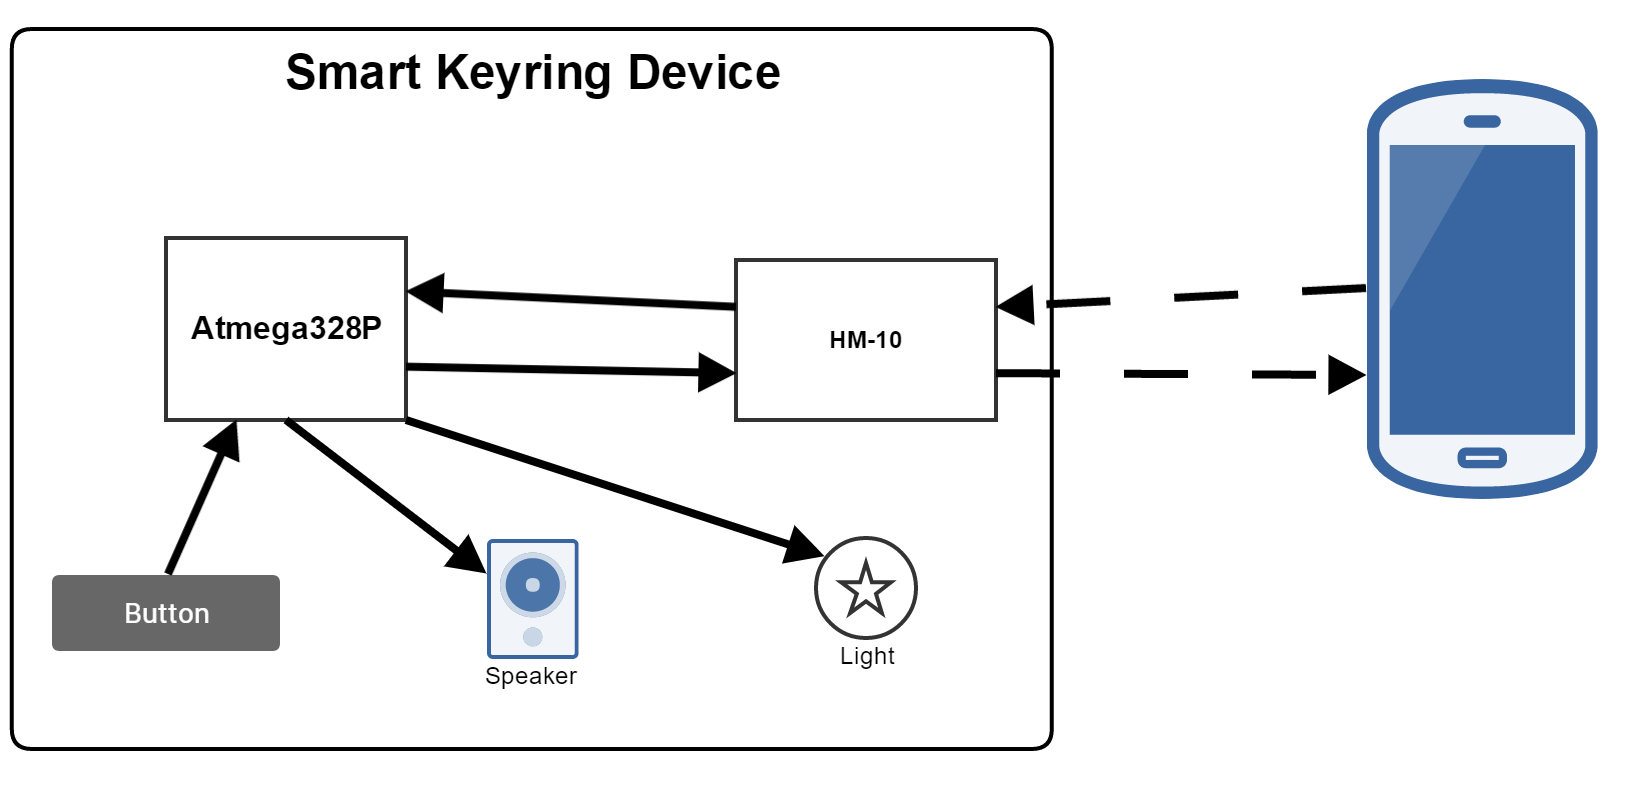
\includegraphics[width=1.0\textwidth]{general}
	\caption[Sơ đồ hoạt động tổng quát]{Sơ đồ hoạt động tổng quát}
	\label{fig: general}
\end{figure}

Như hình \ref{fig: general}, thiết bị Smart Keyring giao tiếp với thiết bị di động thông qua module BLE HM-10 và được điều khiển bởi MCU ATmega328P đảm nhận chức năng quản lý I/O như nút ấn, loa báo hiệu và đèn cũng như là truyền nhận thông điệp với module HM10.

\subsection{Nhận lệnh báo từ thiết bị di động}

Chức năng tìm kiếm thiết bị được kích hoạt bởi thiết bị di động được mô tả ở hình \ref{fig: ring1}.

Trình tự các hoạt động như sau:

(1) Thiết bị di động gửi gói tin với nội dung yêu cầu phát tín hiệu báo tới module HM-10.

(2) MCU ATmega328P nhận gói tin từ module HM-10 bằng giao thức UART với chế độ interrupt.

(3) Loa và đèn báo hiệu được kích hoạt tùy theo nội dung gói tin: kích hoạt cả hai hoặc chỉ kích hoạt đèn báo hiệu

(4*) Nút nhấn có chức năng ngắt chế độ báo hiệu khi cần thiết thông qua interrupt GPIO

\begin{figure}[h]
	\centering    
	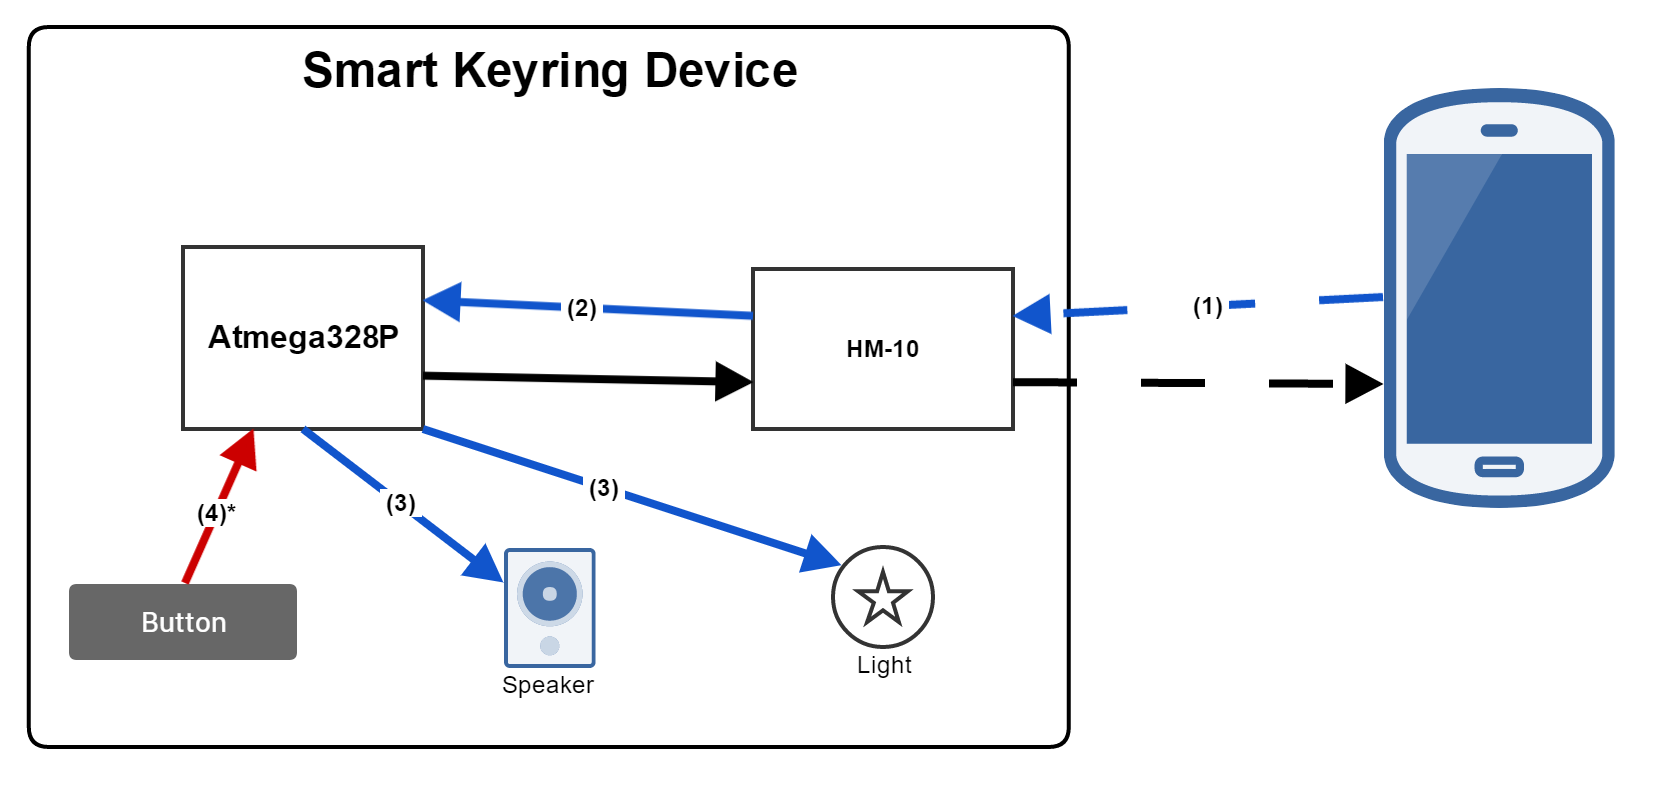
\includegraphics[width=1.0\textwidth]{ring1}
	\caption[Sơ đồ hoạt động khi nhận lệnh báo từ thiết bị di động]{Sơ đồ hoạt động khi nhận lệnh báo từ thiết bị di động}
	\label{fig: ring1}
\end{figure}

Sơ đồ hoạt động trên đúng với chức năng ngắt báo hiệu thiết bị được điều khiển bởi thiết bị di động, chỉ khác tại bước (3) là ngắt loa và đèn và không có bước (4).
\subsection{Kích hoạt thiết bị di động bật chế độ báo hiệu}

Chức năng kích hoạt thiết bị di động bật chế độ báo hiệu được mô tả ở hình \ref{fig: ring2}.

Trình từ các hoạt động như sau:

(1) MCU ATmega328P nhận tín hiệu điều khiển từ nút ấn thông qua interrupt GPIO

(2) Module BLE HM-10 nhận gói tin điều khiển từ MCU ATmega328 thông qua UART

(3) Thiết bị di động nhận gói tin truyền từ Module HM-10 và kích hoạt chế độ báo hiệu

\begin{figure}[h]
	\centering    
	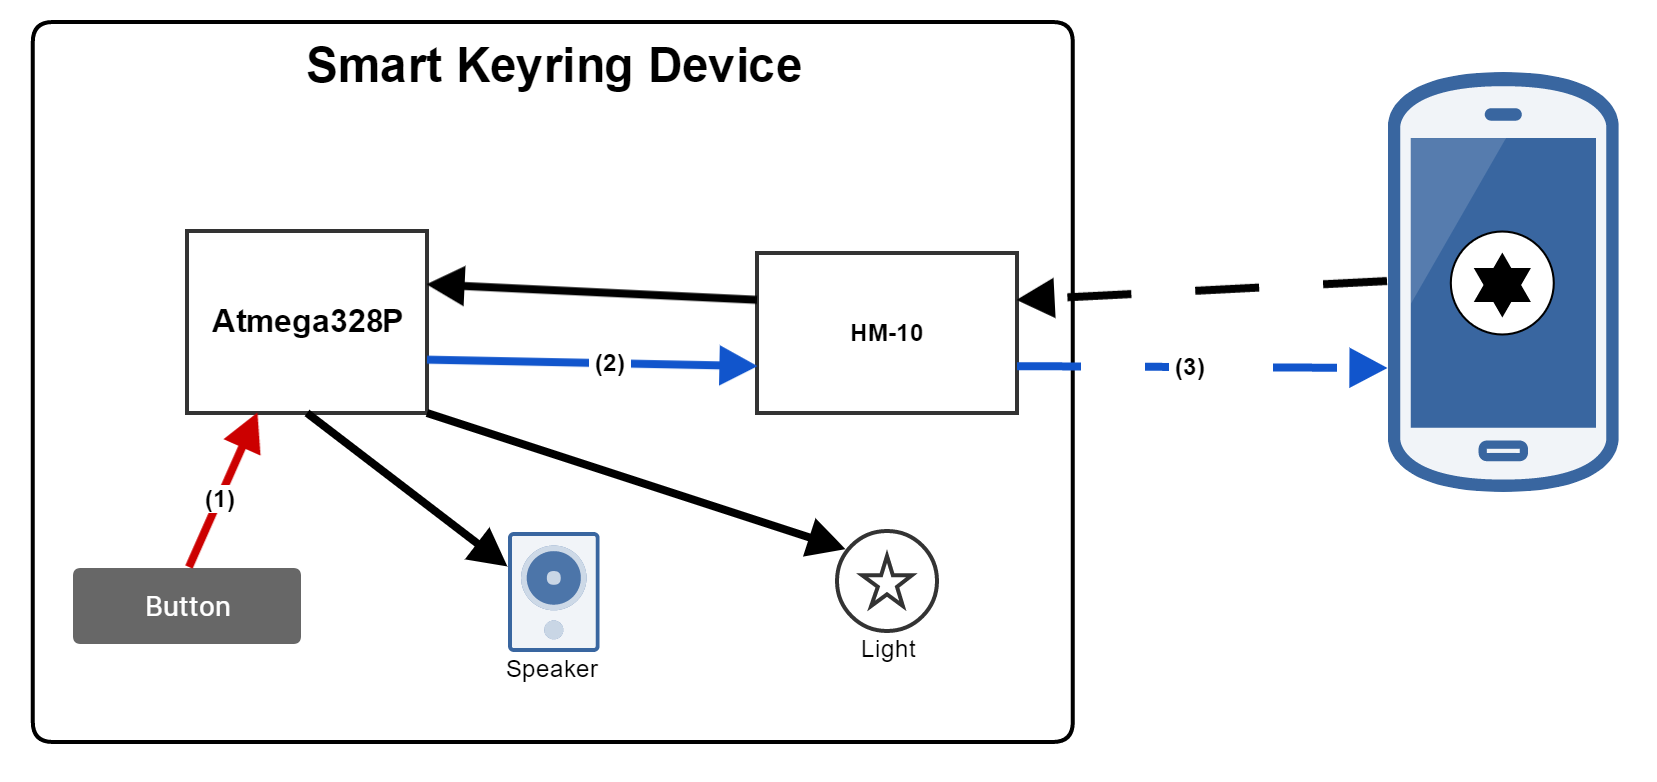
\includegraphics[width=1.0\textwidth]{ring2}
	\caption[Sơ đồ kích hoạt thiết bị di động bật chế độ báo hiệu]{Sơ đồ kích hoạt thiết bị di động bật chế độ báo hiệu}
	\label{fig: ring2}
\end{figure}
\newpage

\subsection{Sơ đồ trạng thái hoạt động khi ngắt kết nối}
%TODO: xem lại phần này
Dựa theo tính năng sản phẩm ở mục \ref{feature}, sơ đồ trạng thái hoạt động được thiết kế ở hình \ref{fig: ble} và \ref{fig: blelost}

	\begin{figure}[H]
		\centering    
		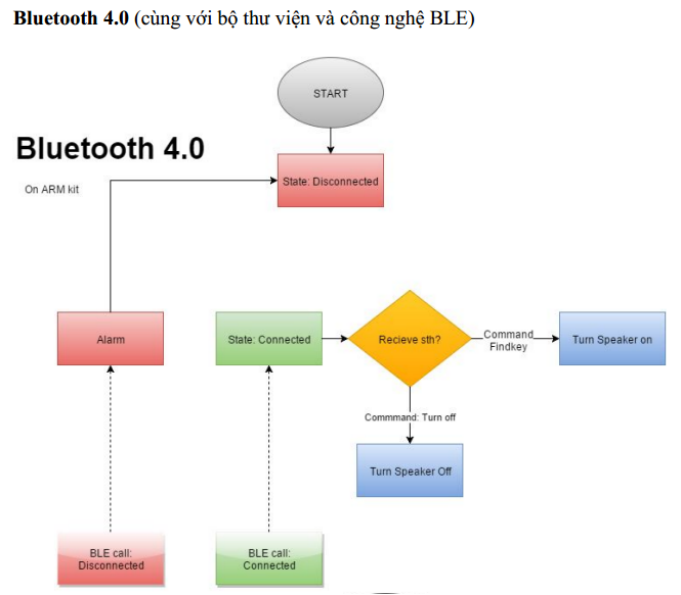
\includegraphics[width=1.0\textwidth]{ble}
		\caption[Sơ đồ trạng thái trên thiết bị Smart Keyring]{Sơ đồ trạng thái trên thiết bị Smart Keyring}
		\label{fig: ble}
	\end{figure}
	
	\begin{figure}[H]
		\centering    
		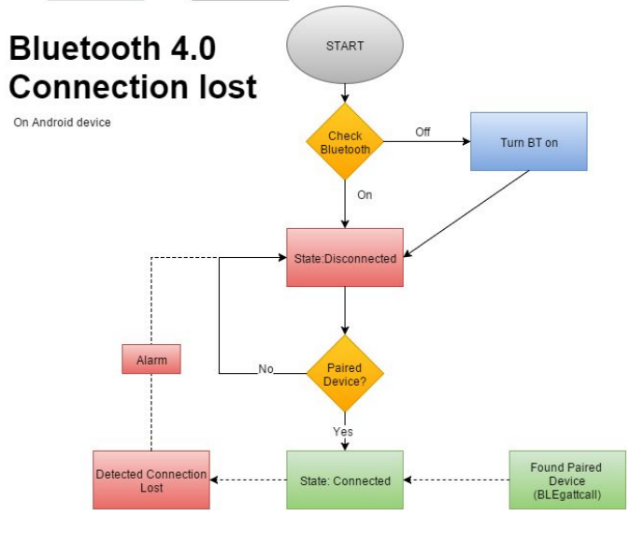
\includegraphics[width=1.0\textwidth]{blelost}
		\caption[Sơ đồ hoạt động trên thiết bị di động]{Sơ đồ hoạt động trên thiết bị di động}
		\label{fig: blelost}
	\end{figure}

\section{Hiện thực phần cứng}
\subsection{Lựa chọn linh kiện và thiết bị phần cứng}

\textit{Sản phẩm hiện thực gồm 3 phần:}

\textbf{Module giao tiếp không dây:}

Tất nhiên yêu cầu tiên quyết của sản phẩm là việc giao tiếp không dây giữa các thiết bị, tiếp theo là việc làm sao để tiết kiệm năng lượng trên từng phần của sản phẩm. Thông qua tìm hiểu, nhóm đã phát hiện ra công nghệ truyền dữ liệu không dây trong khoảng cách ngắn phổ biển nhất hiện nay là công nghệ Bluetooth Low Energy. 

Hiện nay, trên thị trường có rất nhiều loại mẫu mã và thiết kế cho module Bluetooth Low Energy từ nhiều hãng sản xuất khác nhau. Thời gian đầu lúc tiếp cận, nhóm đã lựa chọn mẫu phổ biến nhất trên thị trường hiện nay với giá thành tương đối hợp lí. Đó là module Bluetooth BLE HM-10 của hãng JNHuamao Technology Company có xuất xứ từ Trung Quốc. Sau thời gian thử nghiệm và nghiên cứu với nhiều phiên bản của sản phẩm, nhóm nhận thấy module hoạt động tốt và ổn định, thông số kỹ thuật mà nhà sản xuất cung cấp gần đúng với các thông số kỹ thuật mà nhóm rút ra được trong quá trình thử nghiệm.

\begin{figure}[h]
	\centering    
	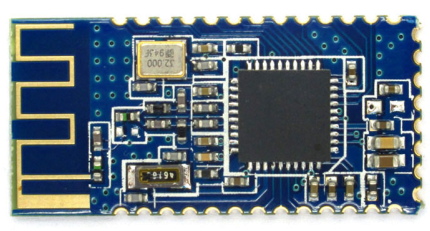
\includegraphics[width=1.0\textwidth]{hm10}
	\caption[Module BLE HM-10]{Module BLE HM-10}
	\label{fig: c2-hm10}
\end{figure}

Thông số kỹ thuật của module: (do nhà sx cung cấp)

• SoC: CC2540/2541 (tùy theo đợt sản xuất)

• BT version: Bluetooth Specification V4.0 BLE.

• Tần số hoạt động: 2.4GHz ISM band.

• RF power: -23dbm, -6dbm, 0dbm, 6dbm.

• Baudrate: hỗ trợ đến 230400, mặc định là 9600.

• Nguồn: +2.5 - 3.3VDC 50mA.

• Dòng tiêu thụ: Active mode 8.5mA, Sleep mod 50-200 uA.

• Thực nghiệm cho thấy module có thể thực hiện truyền nhận trong khoảng cách 20m – 30m( tùy vào thiết bị di động).

\textbf{Vi điều khiện trung tâm:}

Vi điều khiển trung tâm cũng cần thỏa mản một số yêu cầu sau:

• Điện áp hoạt động: 3.3V hoặc ít hơn.

• Có ít nhất 1 kênh giao tiếp UART.

• Tiết kiệm năng lượng nhiều nhất có thể.

• Công cụ lập trình dễ tiếp cận và có bộ thư viện hỗ trợ tương đối đầy đủ.

Với những yêu cầu trên, qua quá trình tìm hiểu và đúc kết kinh nghiệm từ trước, nhóm đã chọn được vi điều khiển thích hợp cho mô hình. Đó là vi điều khiển ATmega328P của hãng Atmel.

\begin{figure}[H]
	\centering    
	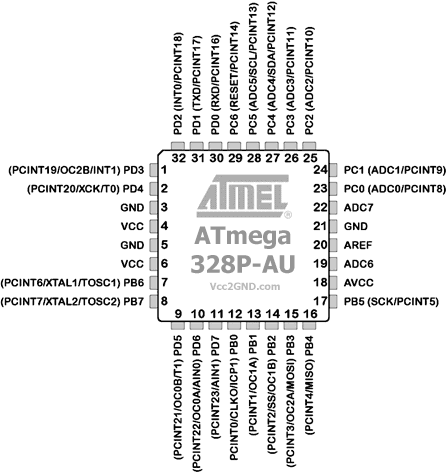
\includegraphics[width=1.0\textwidth]{atmega}
	\caption[MCU ATmega328P]{MCU ATmega328P}
	\label{fig: atmega}
\end{figure}

\textbf{Các thông số kỹ thuật:}

Core:	 AVR 8-bit

Kích thước bộ nhớ FLASH:	 32 KB Flash

Tần số hoạt động tối đa:	 20 MHz

Các chuẩn giao tiếp:	 I²C, SPI, UART/USART

Số lượng cổng GPIO:	 23

Điện áp hoạt động:	 1.8V to 5.5V

\textbf{Các thiết bị xuất nhập:}

• LED nguồn: chức năng báo hiệu khi thiết bị đang hoạt động.

• LED báo hiệu: chức năng bật tắt bằng ánh sáng LED khi có yêu cầu từ thiết bị di động.

• Buzzer: chức năng phát âm thanh khi có yêu cầu từ thiết bị di động.

• Nút bấm: chức năng kích hoạt thiết bị Smart Keyring gửi lệnh cho thiết bị di động báo chuông.

Theo như yêu cầu chức năng ở mục \ref{feature}, schematic được thiết kế như hình \ref{fig: schematic}

	\begin{figure}[H]
		\centering    
		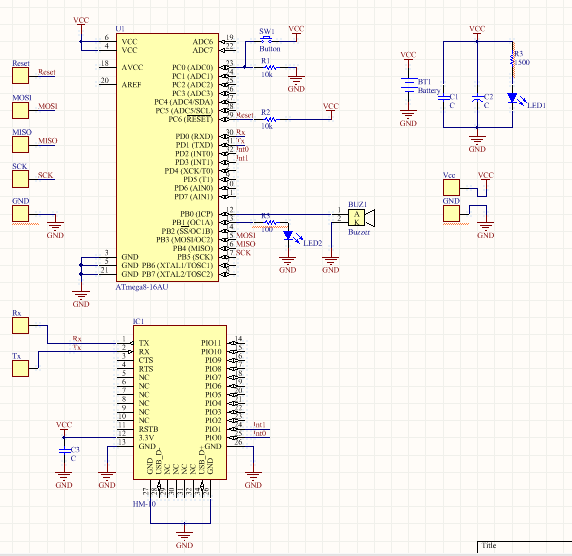
\includegraphics[width=1.0\textwidth]{schematic}
		\caption[Schematic của thiết bị Smart Keyring]{Schematic của thiết bị Smart Keyring}
		\label{fig: schematic}
	\end{figure}
	
Mạch thiết bị thử nghiệm theo schematic như hình \ref{fig: keydraft}

	\begin{figure}[H]
		\centering    
		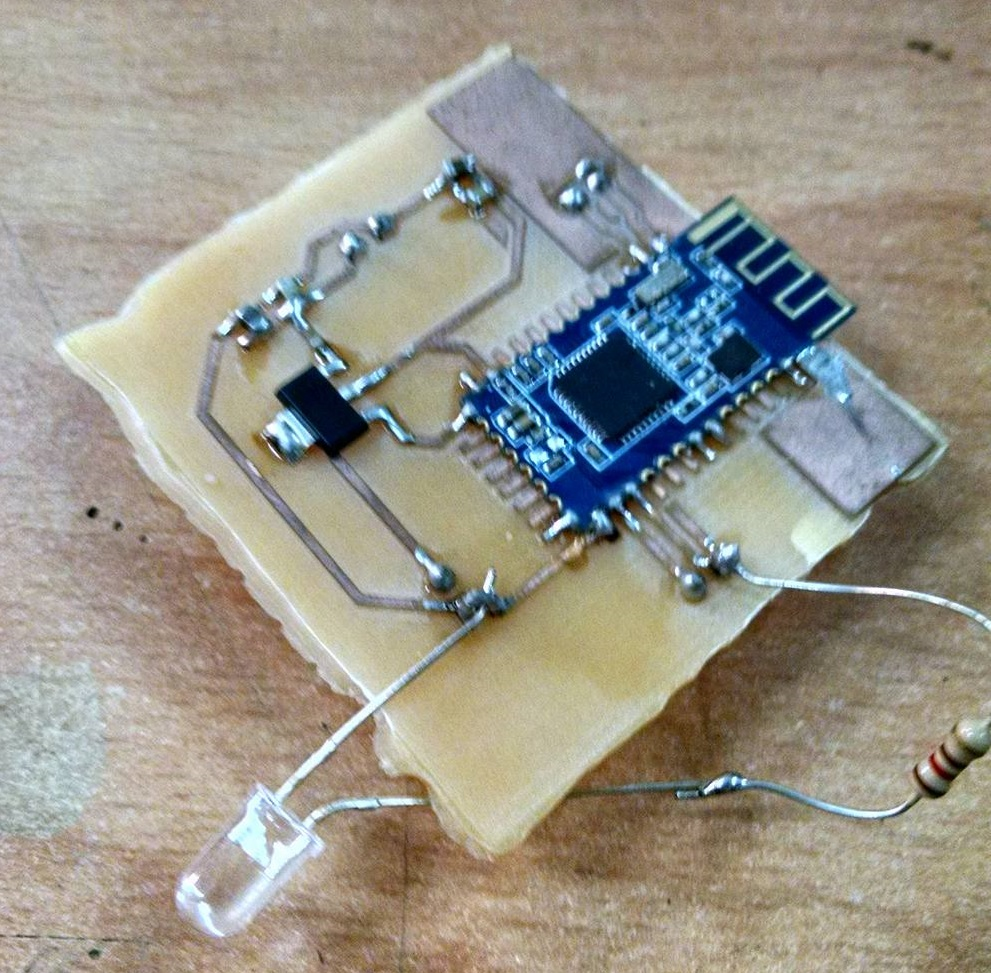
\includegraphics[width=0.5\textwidth]{keydraft}
		\caption[Mạch thử nghiệm]{Mạch thử nghiệm}
		\label{fig: keydraft}
	\end{figure}

Kết quả thử nghiệm giao tiếp và các thiết bị IO hoạt động tốt nên tiến hành đặt mạch và làm mạch chính thức ở hình \ref{fig: key1} và \ref{fig: key2}

	\begin{figure}[H]
		\centering    
		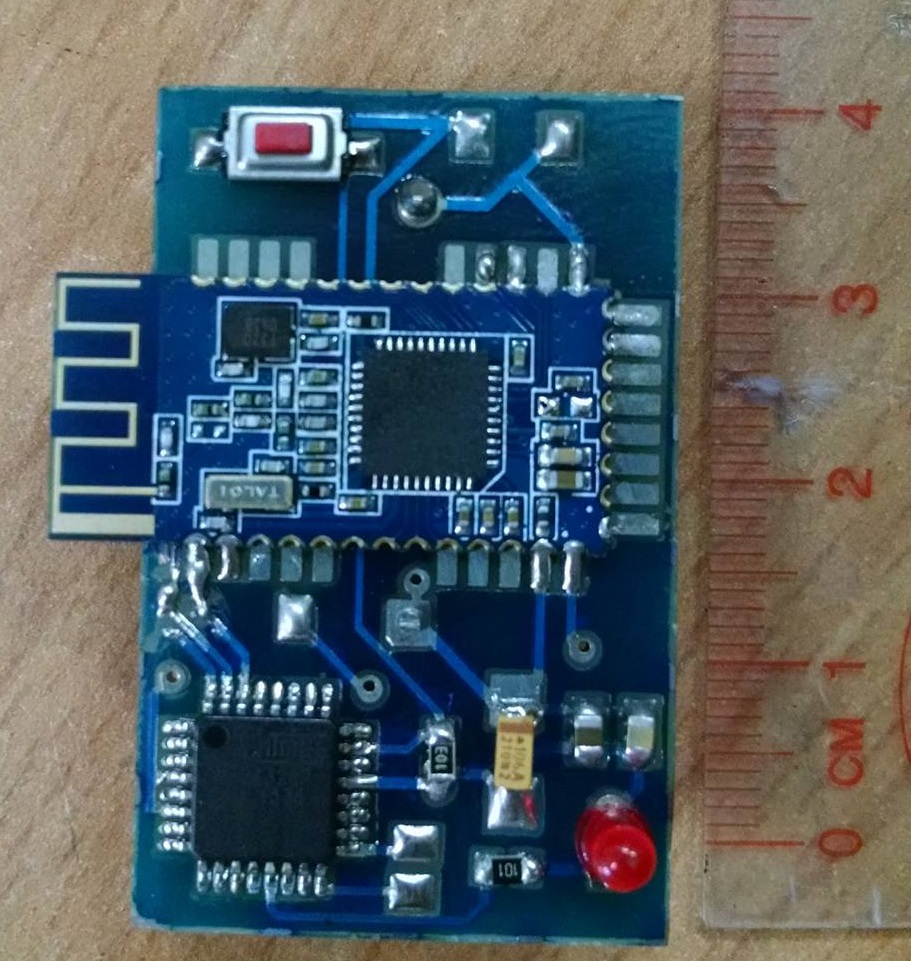
\includegraphics[width=0.5\textwidth]{key1}
		\caption[Mặt trước mạch thiết bị]{Mặt trước mạch thiết bị}
		\label{fig: key1}
	\end{figure}	
	
	\begin{figure}[H]
		\centering    
		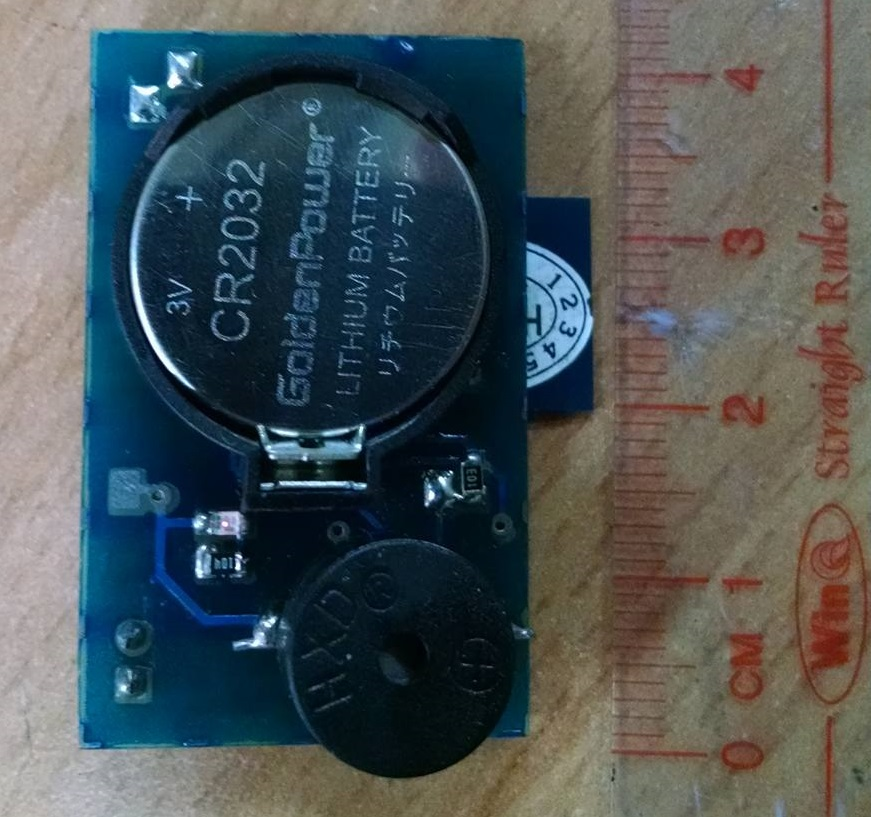
\includegraphics[width=0.5\textwidth]{key2}
		\caption[Mặt sau mạch thiết bị]{Mặt sau mạch thiết bị}
		\label{fig: key2}
	\end{figure}	
	
\subsection{Lập trình firmware cho thiết bị}

Tận dụng tính đơn giản của sản phẩm ứng dụng, các chức năng của sản phẩm được lập trình sao cho việc xử lí các input và output được thực hiện hoàn toàn bằng interrupt. Như vậy, ta sẽ không cần hiện thực thêm chương trình chính và có thể đưa vi điều khiển vào chế độ sleep mode, cụ thể hơn là Idle mode. Từ đó giúp hệ thống tiết kiệm năng lượng hơn.

	\begin{figure}[H]
		\centering    
		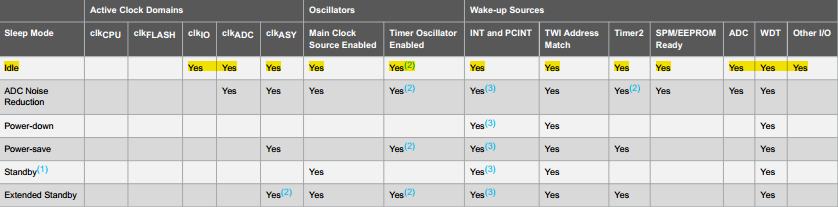
\includegraphics[width=1\textwidth]{sleep}
		\caption[Các chế độ sleep mode khác nhau và khả năng hoạt động của từng chế độ]{Các chế độ sleep mode khác nhau và khả năng hoạt động của từng chế độ}
		\label{fig: sleep}
	\end{figure}
		
Khi MCU đi vào Idle mode, CPU sẽ ngừng hoạt động nhưng các bộ USART, SPI, Timer/Counters, hệ thống Interrupt vẫn sẽ tiếp tục hoạt động.
Idle mode cho phép MCU ‘wake up’ khi xảy ra ngắt ngoài cũng như ngắt trong từ USART Receive, Timer Overflow…

\textbf{Hiện thực interrupt}

Như được đề cập ở trên, việc hiện thực chương trình cho ứng dụng cũng là hiện thực việc xử lí ở các interrupt, bao gồm USART Receive Interrupt và External Inerrupt.

\textbf{USART Receive Interrupt}

\textit{Xảy ra khi nhận được dữ liệu bất kì từ UART:} Dữ liệu này vi điều khiển nhận được thông qua module Bluetooth gửi từ thiết bị di động. Nếu dữ liệu nhận được là ‘R’, chương trình sẽ cho active chân kết nối với chuông. Nếu dữ liệu nhận được là ‘L’, chương trình cho active chân kết nối đến đèn. Ngoài ra, chương trình sẽ không có phản hồi nào khác. Chức năng trên được biểu diễn dưới dạng code:
	\begin{figure}[H]
		\centering    
		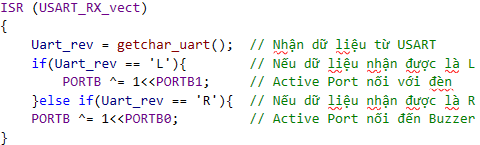
\includegraphics[width=1\textwidth]{int}
		\label{fig: int}
	\end{figure}
	
\textbf{External Inerrupt}

\textit{Xảy ra khi nhận input từ nút nhấn hoặc tín hiệu disconnect từ module Bluetooth):}
Mỗi khi có interrupt từ nút nhấn, chương trình sẽ cho truyền kí tự ‘R’ đến module Bluetooth, từ đó truyền đến thiết bị di động để phát lệnh đỗ chuông.
Khi có interrupt từ module Bluetooth, việc này xảy ra chỉ khi có 1 thiết bị đang kết nối với module Bluetooth đột nhiên mất kết nối. Khi đó, chương trình sẽ điều khiển chân kết nối với chuông để phát tín hiệu mất kết nối được thể hiện bằng đoạn code:

	\begin{figure}[H]
		\centering    
		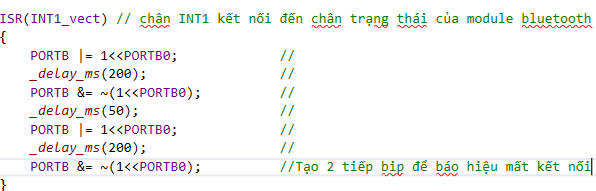
\includegraphics[width=0.8\textwidth]{int2}
		\label{fig: int2}
	\end{figure}

\textbf{Tùy chình baudrate}

Do tính chất hoạt động của sản phẩm đơn giản, hàm lượng dữ liệu truyền nhận giữa các thiết bị ít và không cần đòi hỏi tốc độ quá nhanh, việc hạ thấp baudrate sẽ giúp sản phẩm tiết kiệm năng lượng hơn. Thực tế, mỗi lần cho phát 1 lệnh bất kì giữa 2 thiết bị (smart keyring và tb di động) thì một bên chỉ truyền 1 kí tự (‘L’, ‘R’) để cho biết bên nhận phải phát sáng đèn hay  đỗ chuông. Vì lí do đó, nhóm quyết định hạ thấp baudrate đến mức nhỏ nhất mà module Bluetooth cho phép: 2400Hz
Việc điều chỉnh baudrate cho module Bluetooth khá đơn giản, chỉ cần gửi lệnh theo đúng cú pháp AT+BAUD?
Giá trị thay vào ? sẽ tương ứng với tần số mình cần điều chỉnh

	\begin{figure}[H]
		\centering    
		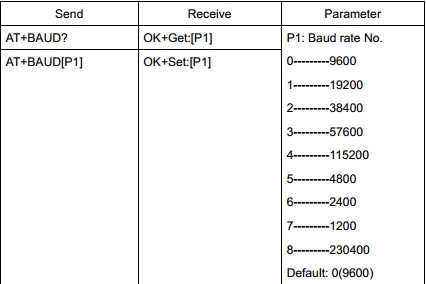
\includegraphics[width=0.7\textwidth]{baud}
		\label{fig: baud}
	\end{figure}

Như vậy, ta chỉ cần gửi lệnh \textbf{AT+BAUD6}. Nếu module Bluetooth phản hồi lại bằng lệnh OK+SET:6 thì ta đã thiết lập thành công \textbf{Baudrate 2400} cho thiết bị

Điều chỉnh tần số xung clock hoạt động của vi điều khiển.
Tốc độ xử lí càng nhanh thì đi đôi với việc tiêu tốn năng lượng càng nhiều. Để hạn chế điều này, nhóm tìm cách hạ thấp tầng số xung clock hoạt động của vi điều khiển đến mức thấp nhất có thể (128KHz). Và với công việc chính của vi điều khiển là giao tiếp UART ở tần số 2400, thì tầng số xung clock này hoàn toàn có thể đáp ứng được theo công thức sau: 

\textbf{UBRRn = FOSC/(16BAUD) – 1}

\textit{UBRRn}: giá trị cần tính để gán vào thanh ghi

\textit{FOSC}: tần số xung clock hoạt động của vi điều khiển

\textit{BAUD}: Baud rate hoạt động khi truyền nhận USART

Thay các giá trị cần tính vào ta được:

\textbf{UBRRn = 128000/(16*2400)-1 = 2.33 > 0}

Do đó việc sử dụng tần số xung clock thấp nhất (128KHz) là hoàn toàn hợp lí, đảm bảo được việc truyền nhận UART trong khi tiết kiệm năng lượng đáng kể so với việc sử dụng tần số cao hơn.
\section{Hiện thực ứng dụng di động trên Android}

\subsection{Các khái niệm trong lập trình BLE trên Android}
\label{sec: bleterm}
Dưới đây là những khái niệm chính về BLE được sử dụng: \cite{deva}

\textbf{Generic Attribute Profile (GATT) -  Cấu hình thuộc tính chung }— Cấu hình GATT là đặc điểm kỹ thuật chung cho việc truyền nhận các gói dữ liệu nhỏ được biết đến như là các "đặc tính" trên đường truyền BLE. Tất cả các cấu hình ứng dụng BLE đều dựa trên GATT.

\textbf{Attribute Protocol (ATT) - Thuộc tính của giao thức}—GATT được xây dựng bên trên lớp ATT, thường được nhắc đến là GATT/ATT. ATT được tối ưu hóa trên các thiết bị BLE và sử dụng ít dữ liệu nhất có thể. Các thuộc tính này được định danh duy nhất bởi Universally Unique Identifier (UUID), là 1 chuỗi định danh dưới chuẩn 128-bit để định danh thông tin duy nhất. Các thuộc tính được truyền bởi ATT được định dạng dưới các characteristics và services.

\textbf{Characteristic -  Đặc tính}— Bao gồm một giá trị và 0-n các khóa để miêu tả giá trị của đặc tính. Một đặc tính có thể xem như là 1 kiểu tương tự như lớp.

\textbf{Descriptor - Khóa mô tả}— Khoá mô tả được xác định để miêu tả giá trị đặc tính. Thí dụ, một khóa mô tả có thể đọc được bởi con người, thuộc phạm vi giá trị của đặc tính hoặc một giá trị đo cụ thể của một giá trị đặc tính nào đó.

\textbf{Service - Dịch vụ}— Service là một gói tổng hợp các đặc tính. Ví dụ, ta có thể có dịch vụ gọi là "Theo dõi nhịp tim" vừa bao gồm các đặc tính như "đo nhịp tim". Danh sách các cấu hình GATT và dịch vụ có thể tìm thấy tại bluetooth.org.

\subsection{Phát triển ứng dụng Android}
%TODO: bổ sung hình giao diện ứng dụng
Ứng dụng Android được phát triển từ nguồn ứng dụng mở android-BluetoothLeGatt\cite{blegatt} được cung cấp bởi Google. Ứng dụng này có chức năng demo thiết lập kết nối và nhận dữ liệu theo chuẩn BLE.

Nhóm chúng tôi trong quá trình tìm hiểu đã nhận thấy phù hợp với đề tài và có thể phát triển chức năng cảnh báo khi mất kết nối và báo hiệu để thiết bị Smart Keyring kích hoạt buzzer/led.

%TODO: bỏ các file code và chức năng

Ứng dụng lập trình dựa theo 4 file chính:

\textit{DeviceScanActivity.java:} chức năng tìm kiếm và hiện thị thiết bị BLE

\textit{DeviceControlActivity.java:} chức năng quản lý kết nối và hiển thị các thông tin về trạng thái kết nối và các service đang có.

\textit{BluetoothLeService.java:} quản lý và điều khiển các service

Cơ chế hoạt động của lệnh gửi ký tự qua BLE trên Android:

\begin{lstlisting}
	// BluetoothLeService.java
    public void ring(){
	    char sendC = 'R'; // gan ky tu can gui la 'R'
	    mGattCharacteristics.setValue(String.valueOf(sendC)); // gan ky tu can gui cho characteristic
	    mBluetoothGatt.writeCharacteristic(mGattCharacteristics); // gui ky tu thong qua GATT BLE
	    Log.d("Ring function Call", "Service");
    }
\end{lstlisting}

Xử lý khi mất kết nối: các hoạt động khi kết nối và mất kết nối được quản lý với \textbf{BroadcastReceiver()} bao gồm các giá trị \textbf{BluetoothLeService}. Khi các giá trị này thay đổi thì sẽ dẫn tới các hoạt động tương ứng:

\begin{lstlisting}
	// DeviceControlActivity.java
 BroadcastReceiver() {
  	@Override
  	public void onReceive(Context context, Intent intent) {
  		if (BluetoothLeService.ACTION_GATT_CONNECTED.equals(action)) {
  			mConnected = true;
  			updateConnectionState(R.string.connected);
  			invalidateOptionsMenu();
  		} else if (BluetoothLeService.ACTION_GATT_DISCONNECTED.equals(action)){
	  		mp=MediaPlayer.create(this,R.raw.noti);
	  		mp.start();
  		}
	};
\end{lstlisting}
Và giao diện ứng dụng được thiết kế:

	\begin{figure}[H]
		\centering    
		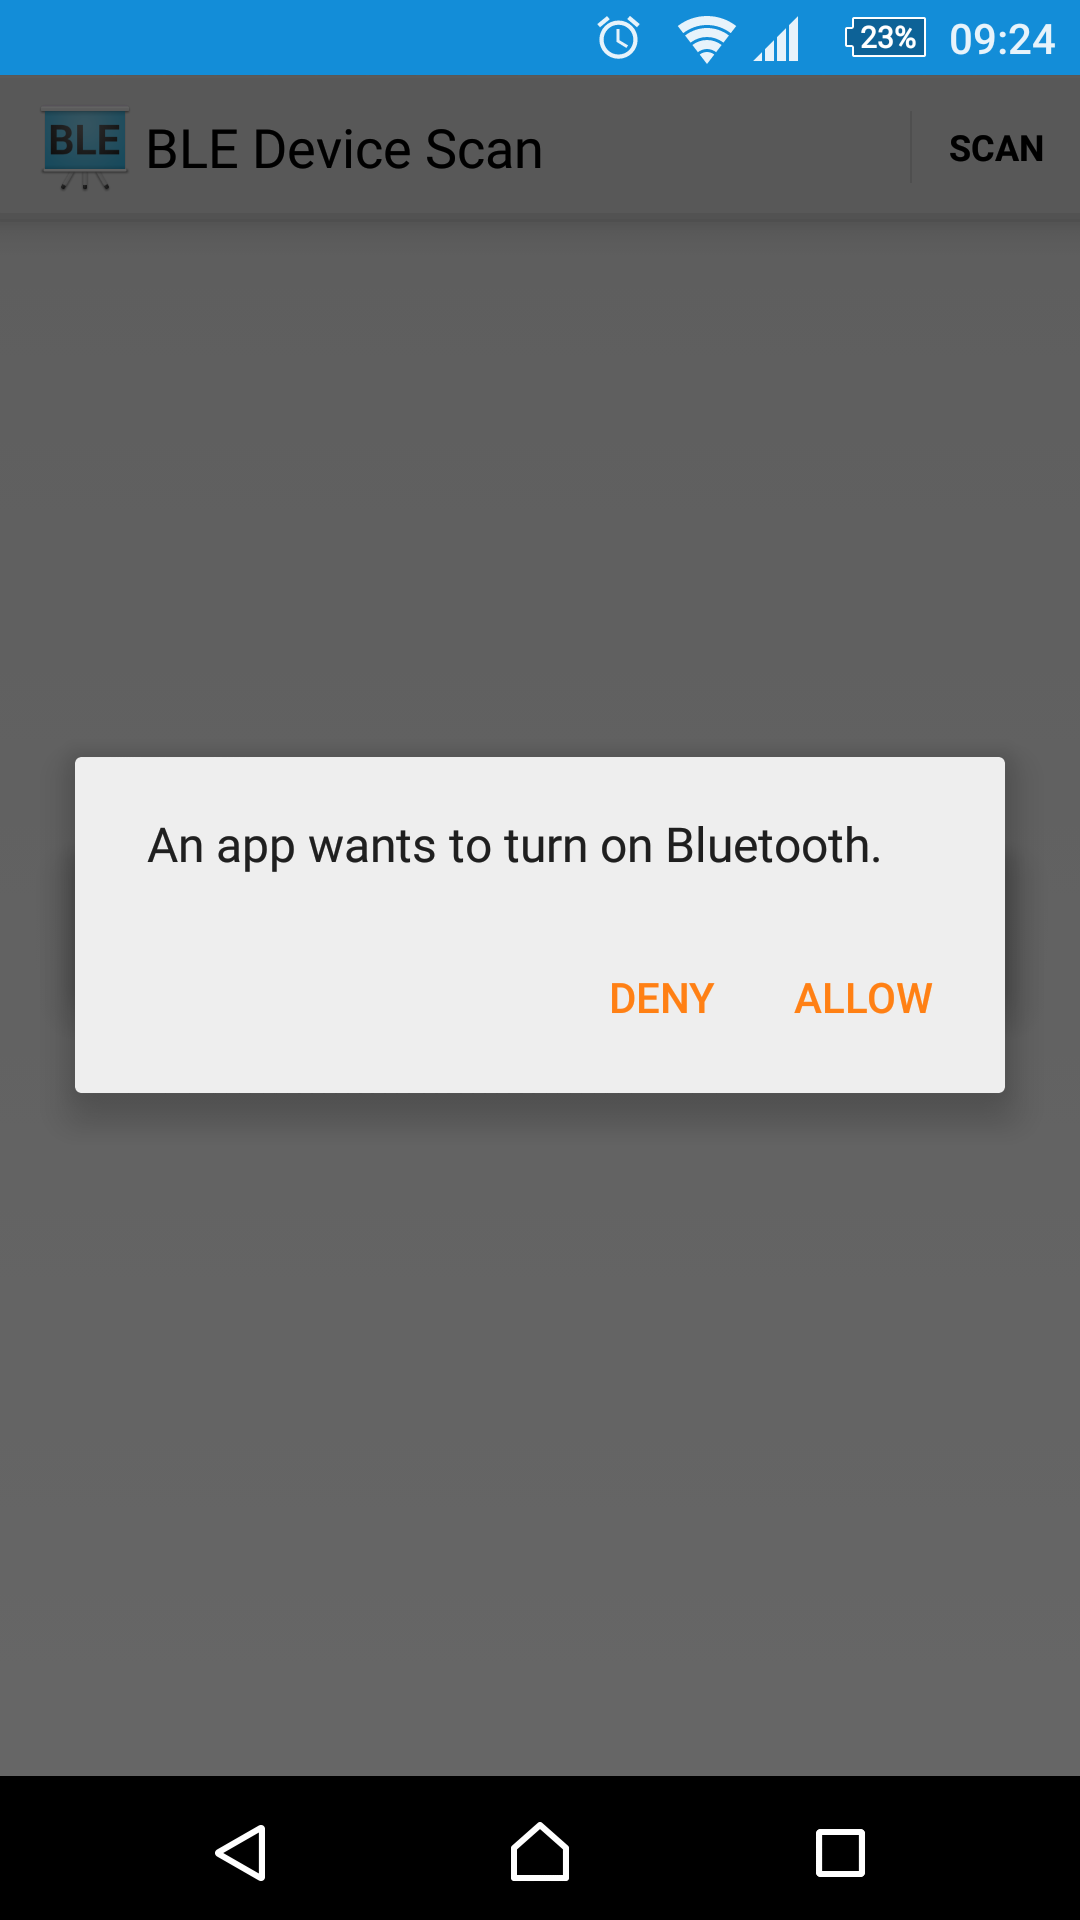
\includegraphics[width=0.6\textwidth]{androidoff}
		\caption[Giao diện kiểm tra BLE]{Giao diện kiểm tra BLE}
		\label{fig: androidoff}
	\end{figure}
Khi khởi động ứng dụng di động, chương trình sẽ kiểm tra thiết bị di động đã bật chế độ Bluetooth chưa và chọn để bắt đầu sử dụng như hình \ref{fig: androidoff}

Nếu thiết bị di động đã bật sẵn chế độ kết nối Bluetooth thì giao diện \ref{fig: androidoff} sẽ không hiện ra.

	\begin{figure}[H]
		\centering    
		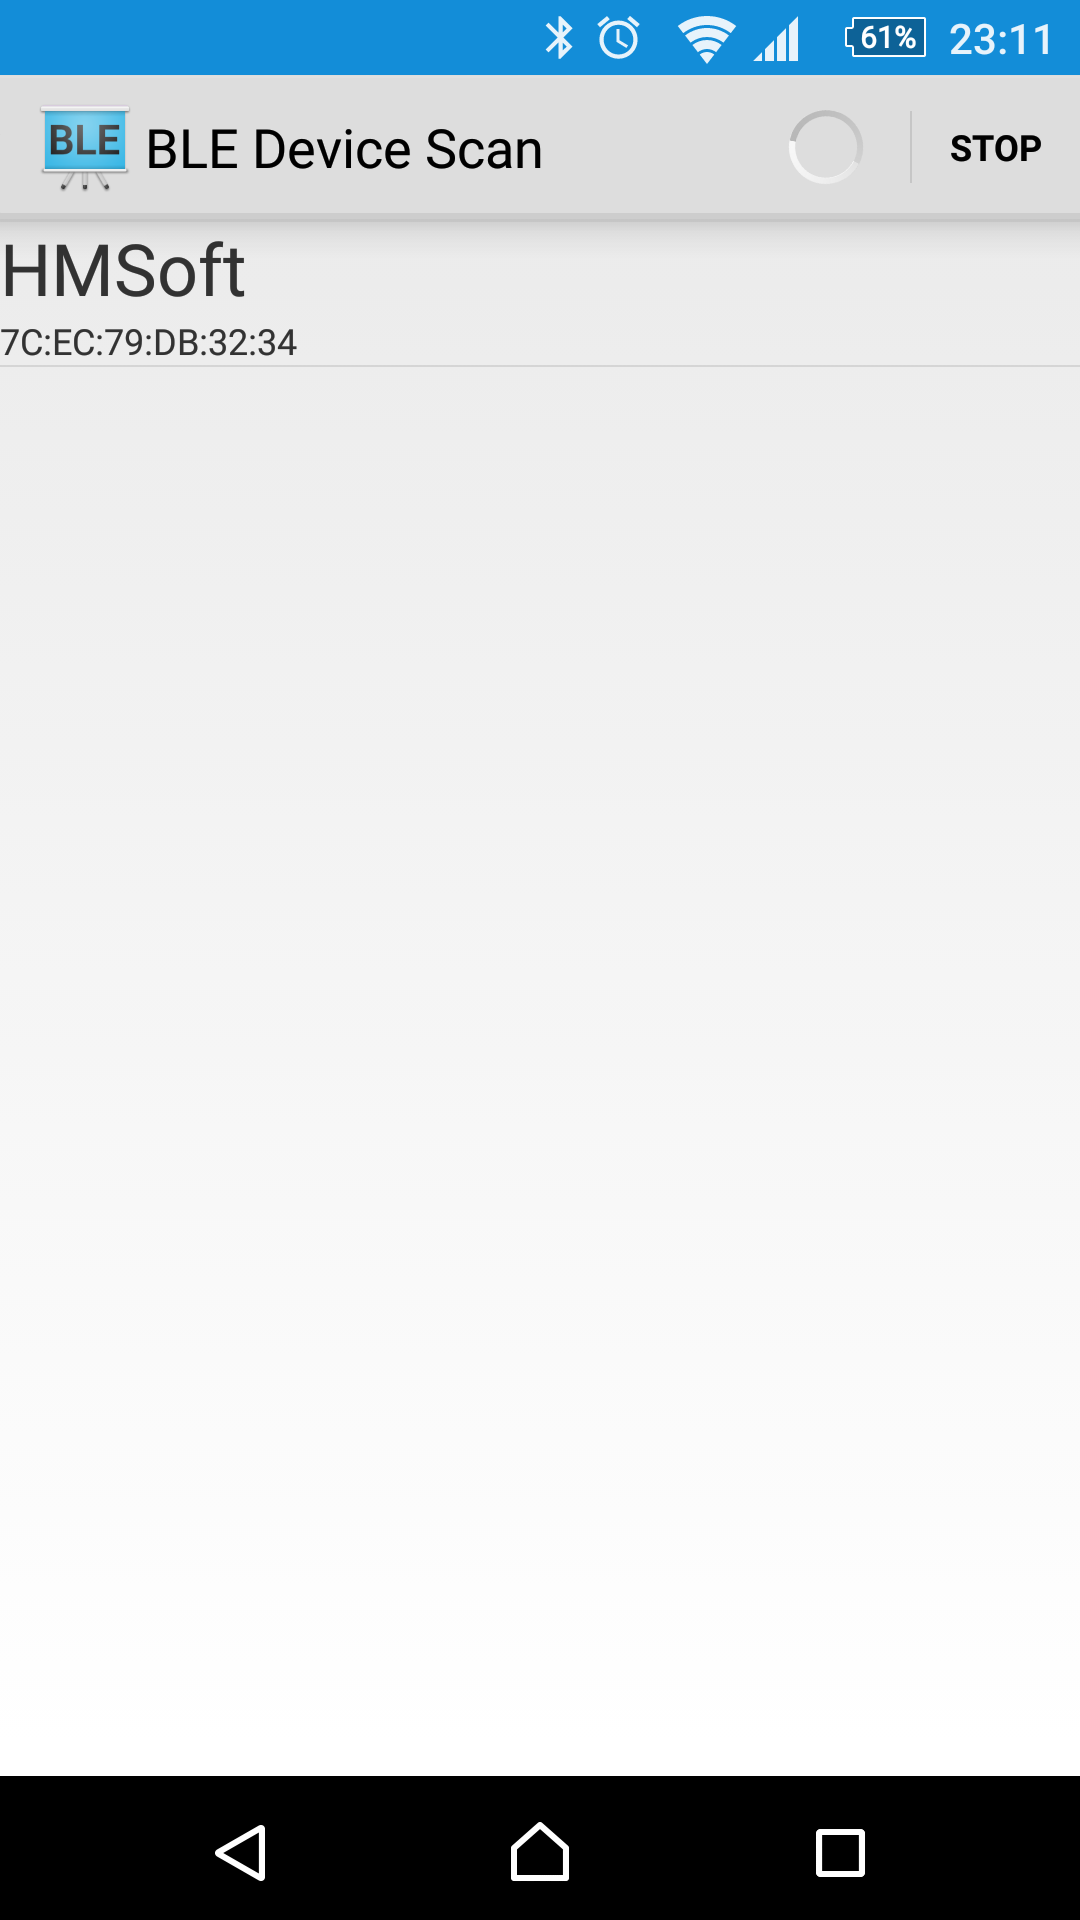
\includegraphics[width=0.6\textwidth]{android1}
		\caption[Giao diện scan thiết bị BLE]{Giao diện scan thiết bị BLE}
		\label{fig: android1}
	\end{figure}
Sau đó ta chọn thiết bị BLE để kết nối, ở đây thiết bị Smart Keyring sử dụng module HM-10 với thiết lập tên hiển thị mặc định là HMSoft. 
	\begin{figure}[H]
		\centering    
		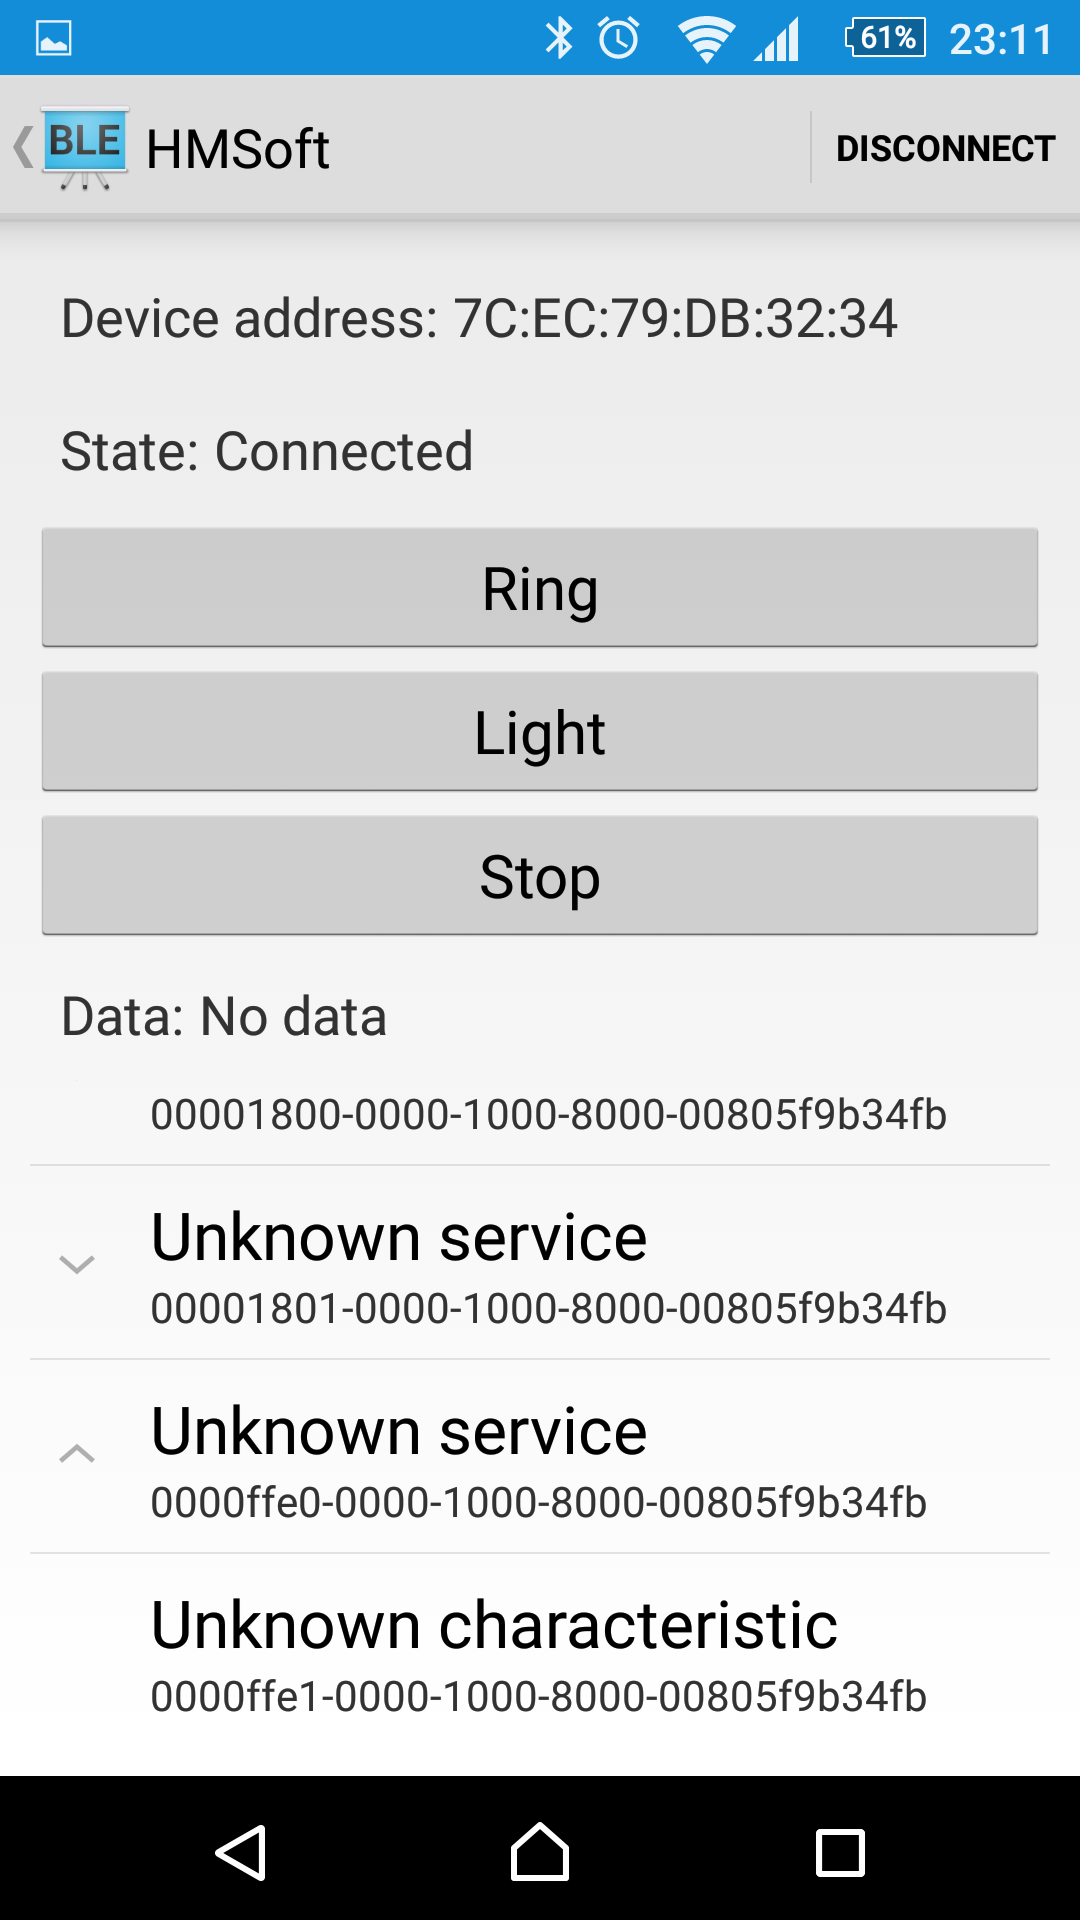
\includegraphics[width=0.6\textwidth]{android2}
		\caption[Giao diện chính của ứng dụng di động]{Giao diện chính của ứng dụng di động}
		\label{fig: android2}
	\end{figure}
	
	Sau khi kết nối, chúng ta sẽ có những thông tin như:
	
	• Device address: địa chỉ MAC của chip CC2540/2541.
	
	• State: Connected hoặc Disconnected -  báo trạng thái kết nối giữa ứng dụng và thiết bị.
	
	• Các service là các characteristic (xem thêm tại \ref{sec: bleterm} ): vì ứng dụng di động đang trong quá trình tìm hiểu và phát triển nên hiển thị các uuid để dễ theo dõi.
	
	Ngoài ra còn có các nút chức năng:
	
	• Ring: gửi yêu cầu bật/tắt báo hiệu bằng buzzer tới thiết bị Smart Keyring.
	
	• Light: gửi yêu cầu bật/tắt báo hiệu bằng LED tới thiết bị Smart Keyring.
	
	• Stop: tắt báo hiệu bằng âm thanh trên thiết bị di động sau khi mất kết nối với thiết bị Smart Keyring.
	
	Để sử dụng các chức năng trên, ta cần chọn service \textbf{0000ffe0-0000-1000-8000-00805f9b34fb} và characteristic \textbf{0000ffe1-0000-1000-8000-00805f9b34fb} - tức là service và characteristic của chức năng đọc truyền nhận dữ liệu thông qua kết nối Bluetooth.

\textit{Source code có thể xem tại: } https://github.com/MrWhoz/ble-smartlkey
	%Demo ứng dụng và đề tài xem thêm tại: 
	%TODO: bỏ link utube